% Options for packages loaded elsewhere
\PassOptionsToPackage{unicode}{hyperref}
\PassOptionsToPackage{hyphens}{url}
\PassOptionsToPackage{dvipsnames,svgnames,x11names}{xcolor}
%
\documentclass[
  letterpaper,
  DIV=11,
  numbers=noendperiod]{scrartcl}

\usepackage{amsmath,amssymb}
\usepackage{iftex}
\ifPDFTeX
  \usepackage[T1]{fontenc}
  \usepackage[utf8]{inputenc}
  \usepackage{textcomp} % provide euro and other symbols
\else % if luatex or xetex
  \usepackage{unicode-math}
  \defaultfontfeatures{Scale=MatchLowercase}
  \defaultfontfeatures[\rmfamily]{Ligatures=TeX,Scale=1}
\fi
\usepackage{lmodern}
\ifPDFTeX\else  
    % xetex/luatex font selection
\fi
% Use upquote if available, for straight quotes in verbatim environments
\IfFileExists{upquote.sty}{\usepackage{upquote}}{}
\IfFileExists{microtype.sty}{% use microtype if available
  \usepackage[]{microtype}
  \UseMicrotypeSet[protrusion]{basicmath} % disable protrusion for tt fonts
}{}
\makeatletter
\@ifundefined{KOMAClassName}{% if non-KOMA class
  \IfFileExists{parskip.sty}{%
    \usepackage{parskip}
  }{% else
    \setlength{\parindent}{0pt}
    \setlength{\parskip}{6pt plus 2pt minus 1pt}}
}{% if KOMA class
  \KOMAoptions{parskip=half}}
\makeatother
\usepackage{xcolor}
\setlength{\emergencystretch}{3em} % prevent overfull lines
\setcounter{secnumdepth}{-\maxdimen} % remove section numbering
% Make \paragraph and \subparagraph free-standing
\makeatletter
\ifx\paragraph\undefined\else
  \let\oldparagraph\paragraph
  \renewcommand{\paragraph}{
    \@ifstar
      \xxxParagraphStar
      \xxxParagraphNoStar
  }
  \newcommand{\xxxParagraphStar}[1]{\oldparagraph*{#1}\mbox{}}
  \newcommand{\xxxParagraphNoStar}[1]{\oldparagraph{#1}\mbox{}}
\fi
\ifx\subparagraph\undefined\else
  \let\oldsubparagraph\subparagraph
  \renewcommand{\subparagraph}{
    \@ifstar
      \xxxSubParagraphStar
      \xxxSubParagraphNoStar
  }
  \newcommand{\xxxSubParagraphStar}[1]{\oldsubparagraph*{#1}\mbox{}}
  \newcommand{\xxxSubParagraphNoStar}[1]{\oldsubparagraph{#1}\mbox{}}
\fi
\makeatother

\usepackage{color}
\usepackage{fancyvrb}
\newcommand{\VerbBar}{|}
\newcommand{\VERB}{\Verb[commandchars=\\\{\}]}
\DefineVerbatimEnvironment{Highlighting}{Verbatim}{commandchars=\\\{\}}
% Add ',fontsize=\small' for more characters per line
\usepackage{framed}
\definecolor{shadecolor}{RGB}{241,243,245}
\newenvironment{Shaded}{\begin{snugshade}}{\end{snugshade}}
\newcommand{\AlertTok}[1]{\textcolor[rgb]{0.68,0.00,0.00}{#1}}
\newcommand{\AnnotationTok}[1]{\textcolor[rgb]{0.37,0.37,0.37}{#1}}
\newcommand{\AttributeTok}[1]{\textcolor[rgb]{0.40,0.45,0.13}{#1}}
\newcommand{\BaseNTok}[1]{\textcolor[rgb]{0.68,0.00,0.00}{#1}}
\newcommand{\BuiltInTok}[1]{\textcolor[rgb]{0.00,0.23,0.31}{#1}}
\newcommand{\CharTok}[1]{\textcolor[rgb]{0.13,0.47,0.30}{#1}}
\newcommand{\CommentTok}[1]{\textcolor[rgb]{0.37,0.37,0.37}{#1}}
\newcommand{\CommentVarTok}[1]{\textcolor[rgb]{0.37,0.37,0.37}{\textit{#1}}}
\newcommand{\ConstantTok}[1]{\textcolor[rgb]{0.56,0.35,0.01}{#1}}
\newcommand{\ControlFlowTok}[1]{\textcolor[rgb]{0.00,0.23,0.31}{\textbf{#1}}}
\newcommand{\DataTypeTok}[1]{\textcolor[rgb]{0.68,0.00,0.00}{#1}}
\newcommand{\DecValTok}[1]{\textcolor[rgb]{0.68,0.00,0.00}{#1}}
\newcommand{\DocumentationTok}[1]{\textcolor[rgb]{0.37,0.37,0.37}{\textit{#1}}}
\newcommand{\ErrorTok}[1]{\textcolor[rgb]{0.68,0.00,0.00}{#1}}
\newcommand{\ExtensionTok}[1]{\textcolor[rgb]{0.00,0.23,0.31}{#1}}
\newcommand{\FloatTok}[1]{\textcolor[rgb]{0.68,0.00,0.00}{#1}}
\newcommand{\FunctionTok}[1]{\textcolor[rgb]{0.28,0.35,0.67}{#1}}
\newcommand{\ImportTok}[1]{\textcolor[rgb]{0.00,0.46,0.62}{#1}}
\newcommand{\InformationTok}[1]{\textcolor[rgb]{0.37,0.37,0.37}{#1}}
\newcommand{\KeywordTok}[1]{\textcolor[rgb]{0.00,0.23,0.31}{\textbf{#1}}}
\newcommand{\NormalTok}[1]{\textcolor[rgb]{0.00,0.23,0.31}{#1}}
\newcommand{\OperatorTok}[1]{\textcolor[rgb]{0.37,0.37,0.37}{#1}}
\newcommand{\OtherTok}[1]{\textcolor[rgb]{0.00,0.23,0.31}{#1}}
\newcommand{\PreprocessorTok}[1]{\textcolor[rgb]{0.68,0.00,0.00}{#1}}
\newcommand{\RegionMarkerTok}[1]{\textcolor[rgb]{0.00,0.23,0.31}{#1}}
\newcommand{\SpecialCharTok}[1]{\textcolor[rgb]{0.37,0.37,0.37}{#1}}
\newcommand{\SpecialStringTok}[1]{\textcolor[rgb]{0.13,0.47,0.30}{#1}}
\newcommand{\StringTok}[1]{\textcolor[rgb]{0.13,0.47,0.30}{#1}}
\newcommand{\VariableTok}[1]{\textcolor[rgb]{0.07,0.07,0.07}{#1}}
\newcommand{\VerbatimStringTok}[1]{\textcolor[rgb]{0.13,0.47,0.30}{#1}}
\newcommand{\WarningTok}[1]{\textcolor[rgb]{0.37,0.37,0.37}{\textit{#1}}}

\providecommand{\tightlist}{%
  \setlength{\itemsep}{0pt}\setlength{\parskip}{0pt}}\usepackage{longtable,booktabs,array}
\usepackage{calc} % for calculating minipage widths
% Correct order of tables after \paragraph or \subparagraph
\usepackage{etoolbox}
\makeatletter
\patchcmd\longtable{\par}{\if@noskipsec\mbox{}\fi\par}{}{}
\makeatother
% Allow footnotes in longtable head/foot
\IfFileExists{footnotehyper.sty}{\usepackage{footnotehyper}}{\usepackage{footnote}}
\makesavenoteenv{longtable}
\usepackage{graphicx}
\makeatletter
\newsavebox\pandoc@box
\newcommand*\pandocbounded[1]{% scales image to fit in text height/width
  \sbox\pandoc@box{#1}%
  \Gscale@div\@tempa{\textheight}{\dimexpr\ht\pandoc@box+\dp\pandoc@box\relax}%
  \Gscale@div\@tempb{\linewidth}{\wd\pandoc@box}%
  \ifdim\@tempb\p@<\@tempa\p@\let\@tempa\@tempb\fi% select the smaller of both
  \ifdim\@tempa\p@<\p@\scalebox{\@tempa}{\usebox\pandoc@box}%
  \else\usebox{\pandoc@box}%
  \fi%
}
% Set default figure placement to htbp
\def\fps@figure{htbp}
\makeatother

\KOMAoption{captions}{tableheading}
\makeatletter
\@ifpackageloaded{caption}{}{\usepackage{caption}}
\AtBeginDocument{%
\ifdefined\contentsname
  \renewcommand*\contentsname{Tabla de contenidos}
\else
  \newcommand\contentsname{Tabla de contenidos}
\fi
\ifdefined\listfigurename
  \renewcommand*\listfigurename{Listado de Figuras}
\else
  \newcommand\listfigurename{Listado de Figuras}
\fi
\ifdefined\listtablename
  \renewcommand*\listtablename{Listado de Tablas}
\else
  \newcommand\listtablename{Listado de Tablas}
\fi
\ifdefined\figurename
  \renewcommand*\figurename{Figura}
\else
  \newcommand\figurename{Figura}
\fi
\ifdefined\tablename
  \renewcommand*\tablename{Tabla}
\else
  \newcommand\tablename{Tabla}
\fi
}
\@ifpackageloaded{float}{}{\usepackage{float}}
\floatstyle{ruled}
\@ifundefined{c@chapter}{\newfloat{codelisting}{h}{lop}}{\newfloat{codelisting}{h}{lop}[chapter]}
\floatname{codelisting}{Listado}
\newcommand*\listoflistings{\listof{codelisting}{Listado de Listados}}
\makeatother
\makeatletter
\makeatother
\makeatletter
\@ifpackageloaded{caption}{}{\usepackage{caption}}
\@ifpackageloaded{subcaption}{}{\usepackage{subcaption}}
\makeatother

\ifLuaTeX
\usepackage[bidi=basic]{babel}
\else
\usepackage[bidi=default]{babel}
\fi
\babelprovide[main,import]{spanish}
% get rid of language-specific shorthands (see #6817):
\let\LanguageShortHands\languageshorthands
\def\languageshorthands#1{}
\usepackage{bookmark}

\IfFileExists{xurl.sty}{\usepackage{xurl}}{} % add URL line breaks if available
\urlstyle{same} % disable monospaced font for URLs
\hypersetup{
  pdftitle={Ejercicio Mínimos Cuadrados},
  pdfauthor={Anthony Contreras},
  pdflang={es},
  colorlinks=true,
  linkcolor={blue},
  filecolor={Maroon},
  citecolor={Blue},
  urlcolor={Blue},
  pdfcreator={LaTeX via pandoc}}


\title{Ejercicio Mínimos Cuadrados}
\author{Anthony Contreras}
\date{}

\begin{document}
\maketitle

\renewcommand*\contentsname{Tabla de Contenidos}
{
\hypersetup{linkcolor=}
\setcounter{tocdepth}{3}
\tableofcontents
}

\section{{[}Participación en clase 11{]} Ejercicio mínimos
cuadrados}\label{participaciuxf3n-en-clase-11-ejercicio-muxednimos-cuadrados}

\subsection{Resolución Prueba 02}\label{resoluciuxf3n-prueba-02}

\begin{itemize}
\tightlist
\item
  Nombre: Anthony Contreras
\item
  Fecha: 26/01/2025
\item
  Curso: Métodos Númericos GR1CC
\end{itemize}

\section{Mínimos Cuadrados}\label{muxednimos-cuadrados}

\begin{itemize}
\tightlist
\item
  Interpole los siguientes conjuntos de datos con la función
  correspondiente. \#\# Link
\end{itemize}

\href{https://github.com/7heAnsw3r/metodos_numericos/blob/main/Participaci\%C3\%B3n/\%5BParticipaci\%C3\%B3n_en_clase_11_Anthony_Contreras.ipynb}{Minimos}

\begin{Shaded}
\begin{Highlighting}[]
\OperatorTok{\%}\NormalTok{load\_ext autoreload}
\end{Highlighting}
\end{Shaded}

\begin{verbatim}
The autoreload extension is already loaded. To reload it, use:
  %reload_ext autoreload
\end{verbatim}

\subsubsection{Conjunto de Datos 1}\label{conjunto-de-datos-1}

\begin{Shaded}
\begin{Highlighting}[]
\NormalTok{xs1 }\OperatorTok{=}\NormalTok{ [}
    \OperatorTok{{-}}\FloatTok{5.0000}\NormalTok{,}
    \OperatorTok{{-}}\FloatTok{3.8889}\NormalTok{,}
    \OperatorTok{{-}}\FloatTok{2.7778}\NormalTok{,}
    \OperatorTok{{-}}\FloatTok{1.6667}\NormalTok{,}
    \OperatorTok{{-}}\FloatTok{0.5556}\NormalTok{,}
    \FloatTok{0.5556}\NormalTok{,}
    \FloatTok{1.6667}\NormalTok{,}
    \FloatTok{2.7778}\NormalTok{,}
    \FloatTok{3.8889}\NormalTok{,}
    \FloatTok{5.0000}\NormalTok{,}
\NormalTok{]}
\NormalTok{ys1 }\OperatorTok{=}\NormalTok{ [}
    \FloatTok{57.2441}\NormalTok{,}
    \FloatTok{33.0303}\NormalTok{,}
    \FloatTok{16.4817}\NormalTok{,}
    \FloatTok{7.0299}\NormalTok{,}
    \FloatTok{0.5498}\NormalTok{,}
    \FloatTok{0.7117}\NormalTok{,}
    \FloatTok{3.4185}\NormalTok{,}
    \FloatTok{12.1767}\NormalTok{,}
    \FloatTok{24.9167}\NormalTok{,}
    \FloatTok{44.2495}\NormalTok{,}
\NormalTok{]}
\end{Highlighting}
\end{Shaded}

\begin{Shaded}
\begin{Highlighting}[]
\ImportTok{from}\NormalTok{ src }\ImportTok{import}\NormalTok{ ajustar\_min\_cuadrados}
\ImportTok{import}\NormalTok{ numpy }\ImportTok{as}\NormalTok{ np}
\ImportTok{import}\NormalTok{ matplotlib.pyplot }\ImportTok{as}\NormalTok{ plt}
\ImportTok{from}\NormalTok{ sympy }\ImportTok{import}\NormalTok{ symbols, Eq, solve}

\KeywordTok{def}\NormalTok{ der\_parcial\_2(xs: }\BuiltInTok{list}\NormalTok{, ys: }\BuiltInTok{list}\NormalTok{) }\OperatorTok{{-}\textgreater{}} \BuiltInTok{tuple}\NormalTok{[}\BuiltInTok{float}\NormalTok{, }\BuiltInTok{float}\NormalTok{, }\BuiltInTok{float}\NormalTok{, }\BuiltInTok{float}\NormalTok{]:}
\NormalTok{    c\_2 }\OperatorTok{=} \BuiltInTok{sum}\NormalTok{(xi}\OperatorTok{**}\DecValTok{2} \ControlFlowTok{for}\NormalTok{ xi }\KeywordTok{in}\NormalTok{ xs)}
\NormalTok{    c\_1 }\OperatorTok{=} \BuiltInTok{sum}\NormalTok{(xs)}
\NormalTok{    c\_0 }\OperatorTok{=} \BuiltInTok{len}\NormalTok{(xs)}
\NormalTok{    c\_ind }\OperatorTok{=} \BuiltInTok{sum}\NormalTok{(ys)}
    \ControlFlowTok{return}\NormalTok{ (c\_2, c\_1, c\_0, c\_ind)}


\KeywordTok{def}\NormalTok{ der\_parcial\_1(xs: }\BuiltInTok{list}\NormalTok{, ys: }\BuiltInTok{list}\NormalTok{) }\OperatorTok{{-}\textgreater{}} \BuiltInTok{tuple}\NormalTok{[}\BuiltInTok{float}\NormalTok{, }\BuiltInTok{float}\NormalTok{, }\BuiltInTok{float}\NormalTok{, }\BuiltInTok{float}\NormalTok{]:}
\NormalTok{    c\_2 }\OperatorTok{=} \BuiltInTok{sum}\NormalTok{(xi}\OperatorTok{**}\DecValTok{3} \ControlFlowTok{for}\NormalTok{ xi }\KeywordTok{in}\NormalTok{ xs)}
\NormalTok{    c\_1 }\OperatorTok{=} \BuiltInTok{sum}\NormalTok{(xi}\OperatorTok{**}\DecValTok{2} \ControlFlowTok{for}\NormalTok{ xi }\KeywordTok{in}\NormalTok{ xs)}
\NormalTok{    c\_0 }\OperatorTok{=} \BuiltInTok{sum}\NormalTok{(xs)}
\NormalTok{    c\_ind }\OperatorTok{=} \BuiltInTok{sum}\NormalTok{(xi }\OperatorTok{*}\NormalTok{ yi }\ControlFlowTok{for}\NormalTok{ xi, yi }\KeywordTok{in} \BuiltInTok{zip}\NormalTok{(xs, ys))}
    \ControlFlowTok{return}\NormalTok{ (c\_2, c\_1, c\_0, c\_ind)}


\KeywordTok{def}\NormalTok{ der\_parcial\_0(xs: }\BuiltInTok{list}\NormalTok{, ys: }\BuiltInTok{list}\NormalTok{) }\OperatorTok{{-}\textgreater{}} \BuiltInTok{tuple}\NormalTok{[}\BuiltInTok{float}\NormalTok{, }\BuiltInTok{float}\NormalTok{, }\BuiltInTok{float}\NormalTok{, }\BuiltInTok{float}\NormalTok{]:}
\NormalTok{    c\_2 }\OperatorTok{=} \BuiltInTok{sum}\NormalTok{(xi}\OperatorTok{**}\DecValTok{4} \ControlFlowTok{for}\NormalTok{ xi }\KeywordTok{in}\NormalTok{ xs)}
\NormalTok{    c\_1 }\OperatorTok{=} \BuiltInTok{sum}\NormalTok{(xi}\OperatorTok{**}\DecValTok{3} \ControlFlowTok{for}\NormalTok{ xi }\KeywordTok{in}\NormalTok{ xs)}
\NormalTok{    c\_0 }\OperatorTok{=} \BuiltInTok{sum}\NormalTok{(xi}\OperatorTok{**}\DecValTok{2} \ControlFlowTok{for}\NormalTok{ xi }\KeywordTok{in}\NormalTok{ xs)}
\NormalTok{    c\_ind }\OperatorTok{=} \BuiltInTok{sum}\NormalTok{(xi}\OperatorTok{**}\DecValTok{2} \OperatorTok{*}\NormalTok{ yi }\ControlFlowTok{for}\NormalTok{ xi, yi }\KeywordTok{in} \BuiltInTok{zip}\NormalTok{(xs, ys))}
    \ControlFlowTok{return}\NormalTok{ (c\_2, c\_1, c\_0, c\_ind)}

\NormalTok{pars1 }\OperatorTok{=}\NormalTok{ ajustar\_min\_cuadrados(xs1, ys1, gradiente}\OperatorTok{=}\NormalTok{[der\_parcial\_0, der\_parcial\_1, der\_parcial\_2])}
\NormalTok{x }\OperatorTok{=}\NormalTok{ symbols(}\StringTok{\textquotesingle{}x\textquotesingle{}}\NormalTok{)}
\NormalTok{equation }\OperatorTok{=}\NormalTok{ Eq(pars1[}\DecValTok{0}\NormalTok{] }\OperatorTok{*}\NormalTok{ x}\OperatorTok{**}\DecValTok{2} \OperatorTok{+}\NormalTok{ pars1[}\DecValTok{1}\NormalTok{] }\OperatorTok{*}\NormalTok{ x }\OperatorTok{+}\NormalTok{ pars1[}\DecValTok{2}\NormalTok{], }\FloatTok{2.25}\NormalTok{)}
\NormalTok{solutions }\OperatorTok{=}\NormalTok{ solve(equation, x)}
\ControlFlowTok{for}\NormalTok{ solution }\KeywordTok{in}\NormalTok{ solutions:}
    \BuiltInTok{print}\NormalTok{(}\SpecialStringTok{f"x = }\SpecialCharTok{\{}\NormalTok{solution}\SpecialCharTok{.}\NormalTok{evalf()}\SpecialCharTok{\}}\SpecialStringTok{"}\NormalTok{)}
\end{Highlighting}
\end{Shaded}

\begin{verbatim}
[01-26 20:20:09][INFO] Se ajustarán 3 parámetros.
[01-26 20:20:09][INFO] 
[[ 1.01852593e+02  0.00000000e+00  1.00000000e+01  1.99808900e+02]
 [ 0.00000000e+00  1.01852593e+02  0.00000000e+00 -1.14413577e+02]
 [-2.27373675e-13  0.00000000e+00 -7.90113041e+01  5.04294087e+01]]
[01-26 20:20:09][INFO] 
[[ 1.01852593e+02  0.00000000e+00  1.00000000e+01  1.99808900e+02]
 [ 0.00000000e+00  1.01852593e+02  0.00000000e+00 -1.14413577e+02]
 [-2.27373675e-13  0.00000000e+00 -7.90113041e+01  5.04294087e+01]]
x = -0.948805441087225
x = 1.50369543945971
\end{verbatim}

Justamente tenia esta idea en el examen pero no me funciono, mi error
fue en el der\_parcial\_2 sumaba en un ciclo para cada valor lo cual era
erroneo.

\begin{Shaded}
\begin{Highlighting}[]
\CommentTok{\# Datos}
\NormalTok{x1 }\OperatorTok{=}\NormalTok{ np.linspace(}\OperatorTok{{-}}\DecValTok{5}\NormalTok{, }\DecValTok{5}\NormalTok{, }\DecValTok{100}\NormalTok{)}
\NormalTok{y1 }\OperatorTok{=}\NormalTok{ pars1[}\DecValTok{0}\NormalTok{] }\OperatorTok{*}\NormalTok{ x1}\OperatorTok{**}\DecValTok{2} \OperatorTok{+}\NormalTok{ pars1[}\DecValTok{1}\NormalTok{] }\OperatorTok{*}\NormalTok{ x1 }\OperatorTok{+}\NormalTok{ pars1[}\DecValTok{2}\NormalTok{]}

\CommentTok{\# Graficar}
\NormalTok{plt.scatter(xs1, ys1, color}\OperatorTok{=}\StringTok{\textquotesingle{}blue\textquotesingle{}}\NormalTok{, label}\OperatorTok{=}\StringTok{"Puntos"}\NormalTok{, edgecolors}\OperatorTok{=}\StringTok{\textquotesingle{}black\textquotesingle{}}\NormalTok{, s}\OperatorTok{=}\DecValTok{80}\NormalTok{)}
\NormalTok{plt.plot(x1, y1, }\StringTok{\textquotesingle{}r{-}\textquotesingle{}}\NormalTok{, label}\OperatorTok{=}\StringTok{"Interpolación cuadrática"}\NormalTok{, linewidth}\OperatorTok{=}\DecValTok{2}\NormalTok{)}

\CommentTok{\# Personalización}
\NormalTok{plt.xlabel(}\StringTok{"x"}\NormalTok{, fontsize}\OperatorTok{=}\DecValTok{14}\NormalTok{)}
\NormalTok{plt.ylabel(}\StringTok{"y"}\NormalTok{, fontsize}\OperatorTok{=}\DecValTok{14}\NormalTok{)}
\NormalTok{plt.title(}\StringTok{"Ajuste Cuadrático"}\NormalTok{, fontsize}\OperatorTok{=}\DecValTok{16}\NormalTok{)}
\NormalTok{plt.legend(loc}\OperatorTok{=}\StringTok{"upper right"}\NormalTok{)}
\NormalTok{plt.grid(}\VariableTok{True}\NormalTok{, linestyle}\OperatorTok{=}\StringTok{\textquotesingle{}{-}{-}\textquotesingle{}}\NormalTok{, alpha}\OperatorTok{=}\FloatTok{0.7}\NormalTok{)}

\CommentTok{\# Mostrar}
\NormalTok{plt.show()}
\end{Highlighting}
\end{Shaded}

\pandocbounded{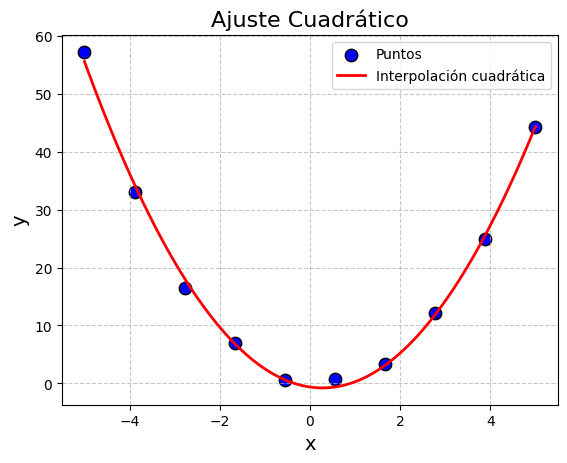
\includegraphics[keepaspectratio]{\%5BParticipación_en_clase_11_Anthony_Contreras_files/figure-pdf/cell-5-output-1.png}}

\begin{Shaded}
\begin{Highlighting}[]
\KeywordTok{def}\NormalTok{ cuadratica(x, pars):}
\NormalTok{    a2, a1, a0 }\OperatorTok{=}\NormalTok{ pars}
    \ControlFlowTok{return}\NormalTok{ a2 }\OperatorTok{*}\NormalTok{ x}\OperatorTok{**}\DecValTok{2} \OperatorTok{+}\NormalTok{ a1 }\OperatorTok{*}\NormalTok{ x }\OperatorTok{+}\NormalTok{ a0}

\KeywordTok{def}\NormalTok{ ajustar\_min\_cuadrados(xs, ys):}
\NormalTok{    A }\OperatorTok{=}\NormalTok{ np.vstack([np.square(xs), xs, np.ones(}\BuiltInTok{len}\NormalTok{(xs))]).T}
\NormalTok{    pars, \_, \_, \_ }\OperatorTok{=}\NormalTok{ np.linalg.lstsq(A, ys, rcond}\OperatorTok{=}\VariableTok{None}\NormalTok{)}
    \ControlFlowTok{return}\NormalTok{ pars}

\NormalTok{pars }\OperatorTok{=}\NormalTok{ ajustar\_min\_cuadrados(xs1, ys1)}
\NormalTok{a2, a1, a0 }\OperatorTok{=}\NormalTok{ pars}

\NormalTok{y\_2\_25 }\OperatorTok{=}\NormalTok{ cuadratica(}\FloatTok{2.25}\NormalTok{, pars)}
\NormalTok{y\_neg\_2\_25 }\OperatorTok{=}\NormalTok{ cuadratica(}\OperatorTok{{-}}\FloatTok{2.25}\NormalTok{, pars)}

\BuiltInTok{print}\NormalTok{(}\SpecialStringTok{f"a2 = }\SpecialCharTok{\{}\NormalTok{a2}\SpecialCharTok{\}}\SpecialStringTok{"}\NormalTok{)}
\BuiltInTok{print}\NormalTok{(}\SpecialStringTok{f"a1 = }\SpecialCharTok{\{}\NormalTok{a1}\SpecialCharTok{\}}\SpecialStringTok{"}\NormalTok{)}
\BuiltInTok{print}\NormalTok{(}\SpecialStringTok{f"a0 = }\SpecialCharTok{\{}\NormalTok{a0}\SpecialCharTok{\}}\SpecialStringTok{"}\NormalTok{)}
\BuiltInTok{print}\NormalTok{(}\SpecialStringTok{f"y(2.25) = }\SpecialCharTok{\{}\NormalTok{y\_2\_25}\SpecialCharTok{\}}\SpecialStringTok{"}\NormalTok{)}
\BuiltInTok{print}\NormalTok{(}\SpecialStringTok{f"y({-}2.25) = }\SpecialCharTok{\{}\NormalTok{y\_neg\_2\_25}\SpecialCharTok{\}}\SpecialStringTok{"}\NormalTok{)}
\end{Highlighting}
\end{Shaded}

\begin{verbatim}
a2 = 2.024410482925084
a1 = -1.1233251295755444
a0 = -0.6382556172537845
y(2.25) = 7.0828409110094785
y(-2.25) = 12.137803994099427
\end{verbatim}

\subsubsection{Conjunto de Datos 2}\label{conjunto-de-datos-2}

\begin{Shaded}
\begin{Highlighting}[]
\NormalTok{xs2 }\OperatorTok{=}\NormalTok{ [}
    \FloatTok{0.0003}\NormalTok{,}
    \FloatTok{0.0822}\NormalTok{,}
    \FloatTok{0.2770}\NormalTok{,}
    \FloatTok{0.4212}\NormalTok{,}
    \FloatTok{0.4403}\NormalTok{,}
    \FloatTok{0.5588}\NormalTok{,}
    \FloatTok{0.5943}\NormalTok{,}
    \FloatTok{0.6134}\NormalTok{,}
    \FloatTok{0.9070}\NormalTok{,}
    \FloatTok{1.0367}\NormalTok{,}
    \FloatTok{1.1903}\NormalTok{,}
    \FloatTok{1.2511}\NormalTok{,}
    \FloatTok{1.2519}\NormalTok{,}
    \FloatTok{1.2576}\NormalTok{,}
    \FloatTok{1.6165}\NormalTok{,}
    \FloatTok{1.6761}\NormalTok{,}
    \FloatTok{2.0114}\NormalTok{,}
    \FloatTok{2.0557}\NormalTok{,}
    \FloatTok{2.1610}\NormalTok{,}
    \FloatTok{2.6344}\NormalTok{,}
\NormalTok{]}
\NormalTok{ys2 }\OperatorTok{=}\NormalTok{ [}
    \FloatTok{1.1017}\NormalTok{,}
    \FloatTok{1.5021}\NormalTok{,}
    \FloatTok{0.3844}\NormalTok{,}
    \FloatTok{1.3251}\NormalTok{,}
    \FloatTok{1.7206}\NormalTok{,}
    \FloatTok{1.9453}\NormalTok{,}
    \FloatTok{0.3894}\NormalTok{,}
    \FloatTok{0.3328}\NormalTok{,}
    \FloatTok{1.2887}\NormalTok{,}
    \FloatTok{3.1239}\NormalTok{,}
    \FloatTok{2.1778}\NormalTok{,}
    \FloatTok{3.1078}\NormalTok{,}
    \FloatTok{4.1856}\NormalTok{,}
    \FloatTok{3.3640}\NormalTok{,}
    \FloatTok{6.0330}\NormalTok{,}
    \FloatTok{5.8088}\NormalTok{,}
    \FloatTok{10.5890}\NormalTok{,}
    \FloatTok{11.5865}\NormalTok{,}
    \FloatTok{11.8221}\NormalTok{,}
    \FloatTok{26.5077}\NormalTok{,}
\NormalTok{]}
\end{Highlighting}
\end{Shaded}

\begin{Shaded}
\begin{Highlighting}[]
\KeywordTok{def}\NormalTok{ exponencial(x, pars):}
\NormalTok{    a, b }\OperatorTok{=}\NormalTok{ pars}
    \ControlFlowTok{return}\NormalTok{ a }\OperatorTok{*}\NormalTok{ np.exp(b }\OperatorTok{*}\NormalTok{ x)}

\KeywordTok{def}\NormalTok{ ajustar\_exponencial(xs, ys):}
\NormalTok{    log\_ys }\OperatorTok{=}\NormalTok{ np.log(ys)}
\NormalTok{    A }\OperatorTok{=}\NormalTok{ np.vstack([xs, np.ones(}\BuiltInTok{len}\NormalTok{(xs))]).T}
\NormalTok{    b, log\_a }\OperatorTok{=}\NormalTok{ np.linalg.lstsq(A, log\_ys, rcond}\OperatorTok{=}\VariableTok{None}\NormalTok{)[}\DecValTok{0}\NormalTok{]}
\NormalTok{    a }\OperatorTok{=}\NormalTok{ np.exp(log\_a)}

    \ControlFlowTok{return}\NormalTok{ a, b}

\NormalTok{pars }\OperatorTok{=}\NormalTok{ ajustar\_exponencial(xs2, ys2)}

\NormalTok{x }\OperatorTok{=}\NormalTok{ np.linspace(}\BuiltInTok{min}\NormalTok{(xs2), }\BuiltInTok{max}\NormalTok{(xs2), }\DecValTok{100}\NormalTok{)}
\NormalTok{y }\OperatorTok{=}\NormalTok{ exponencial(x, pars)}

\CommentTok{\# Graficar ajuste exponencial}
\NormalTok{plt.plot(x, y, color}\OperatorTok{=}\StringTok{"red"}\NormalTok{, linewidth}\OperatorTok{=}\DecValTok{2}\NormalTok{)}
\NormalTok{plt.scatter(xs2, ys2)}
\NormalTok{plt.xlabel(}\StringTok{"x"}\NormalTok{, fontsize}\OperatorTok{=}\DecValTok{14}\NormalTok{)}
\NormalTok{plt.ylabel(}\StringTok{"y"}\NormalTok{, fontsize}\OperatorTok{=}\DecValTok{14}\NormalTok{)}
\NormalTok{plt.title(}\StringTok{"Interpolación: Conjunto de datos 2"}\NormalTok{, fontsize}\OperatorTok{=}\DecValTok{16}\NormalTok{)}
\NormalTok{plt.grid(}\VariableTok{True}\NormalTok{, linestyle}\OperatorTok{=}\StringTok{\textquotesingle{}{-}{-}\textquotesingle{}}\NormalTok{, alpha}\OperatorTok{=}\FloatTok{0.7}\NormalTok{)}
\NormalTok{plt.show()}
\end{Highlighting}
\end{Shaded}

\pandocbounded{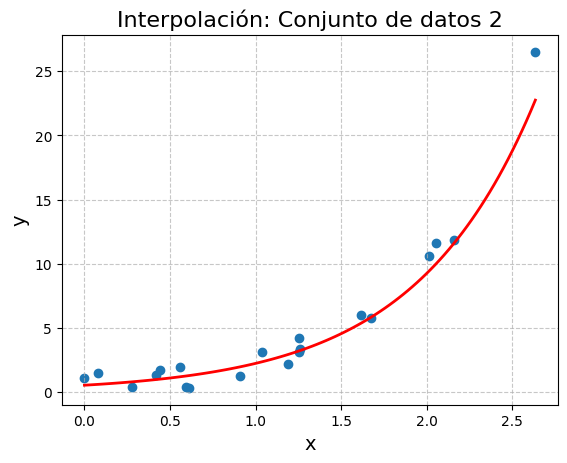
\includegraphics[keepaspectratio]{\%5BParticipación_en_clase_11_Anthony_Contreras_files/figure-pdf/cell-8-output-1.png}}

\begin{Shaded}
\begin{Highlighting}[]
\NormalTok{a, b }\OperatorTok{=}\NormalTok{ pars}

\NormalTok{y\_5 }\OperatorTok{=}\NormalTok{ exponencial(}\DecValTok{5}\NormalTok{, pars)}
\NormalTok{y\_1 }\OperatorTok{=}\NormalTok{ exponencial(}\DecValTok{1}\NormalTok{, pars)}

\BuiltInTok{print}\NormalTok{(}\SpecialStringTok{f"a = }\SpecialCharTok{\{}\NormalTok{a}\SpecialCharTok{\}}\SpecialStringTok{"}\NormalTok{)}
\BuiltInTok{print}\NormalTok{(}\SpecialStringTok{f"b = }\SpecialCharTok{\{}\NormalTok{b}\SpecialCharTok{\}}\SpecialStringTok{"}\NormalTok{)}
\BuiltInTok{print}\NormalTok{(}\SpecialStringTok{f"y(5) = }\SpecialCharTok{\{}\NormalTok{y\_5}\SpecialCharTok{\}}\SpecialStringTok{"}\NormalTok{)}
\BuiltInTok{print}\NormalTok{(}\SpecialStringTok{f"y(1) = }\SpecialCharTok{\{}\NormalTok{y\_1}\SpecialCharTok{\}}\SpecialStringTok{"}\NormalTok{)}
\end{Highlighting}
\end{Shaded}

\begin{verbatim}
a = 0.5440855388147082
b = 1.4171603667055415
y(5) = 650.1174439111649
y(1) = 2.2445646053759507
\end{verbatim}

\section{Conclusiones}\label{conclusiones}

\begin{itemize}
\tightlist
\item
  Uso del Método de Mínimos Cuadrados: El ajuste de los parámetros aa y
  bb se realiza mediante la resolución de un sistema de ecuaciones
  lineales con el método de mínimos cuadrados. Este método es eficiente
  para encontrar los mejores parámetros en el sentido de minimizar el
  error cuadrático entre los valores ajustados y los datos reales. En
  este caso, se usa la función np.linalg.lstsq, que es apropiada para
  resolver este tipo de problemas.
\item
  Una vez encontrados los parámetros aa y bb, se genera una curva
  ajustada para los valores de xx. Esto permite visualizar cómo el
  modelo exponencial se adapta a los datos observados.
\end{itemize}




\end{document}
